% 西北农林科技大学科技类及IT类课程论文文档类(LaTeX模板)
\documentclass[
  % projtype=paper, % 实习类型,可选report(报告)或paper(论文),默认为report
  % output=epub,     % 输出类型,可选print(打印,不显示超链接颜色)
                   %           或epub(电子稿,显示超链接颜色),默认为epub
  ]{nwafuprojrep}

% 载入需要的宏包
\input{settings/packages.tex}
% 进行必要的设置
\input{settings/format.tex}
% 专用术语宏命令
\input{settings/terms.tex}
% 数学符号宏命令
\input{settings/math-commands.tex}

% 设置封面基本信息,\linebreak 前面不要有空格,
% 中文之间的空格无法消除
% 另,在\nwafuset中不可以出现空行
\nwafuset{
  college = {信息工程学院},            % 学院名称
  projname = {面向对象程序设计},       % 实践课程名称
  title = {\LaTeX{}科技排版实习报告},  % 实习报告题目
  stuno = {2019012971},              % 学号
  author = {何志杰},             % 姓名
  major = {软件工程},          % 专业
  classid = {1903},                   % 班级(只填写数字,不要有其它内容)
  adviser = {魏蕾},                   % 指导教师姓名
  startdate = {2020年8月24日},        % 实践起始日期
  enddate = {9月4日},        % 实践结束日期
}

%biblatex宏包的参考文献数据源加载方式
\addbibresource[location=local]{bib/example.bib}
\begin{document} %在document环境中撰写文档

%%%%%%%%%%%%%%%%%%%%%%%%%%%%%%%%%%%%%%%%
% 封面及目录,无需改动此处代码
% 面页,需要在导言区用\nwafuset命令填写基本信息
\makecover
% 目录
\tableofcontents
\cleardoublepage
% 设置正文页眉页脚格式,并重新设置页码为1
\pagestyle{main}% 无页眉,页码在页脚居中
%%%%%%%%%%%%%%%%%%%%%%%%%%%%%%%%%%%%%%%%


% 排版摘要
% 摘要内容
\begin{abstract}
  针对现实生活中人工登记学生信息繁琐、数据易丢失等问题,我们基于Qt5制作了有图形化GUI界面的学生信息管理系统,具有易登记、易保存信息等特点。
  本系统基于面向对象程序设计,实现了基本的学生信息增删改查功能,还额外添加了学生学号、成绩排序等功能。数据的存储采用文件来实现,可移植性能强。
\end{abstract}
% 关键词内容(不同关键字,请用英文","分割)
\keywords{学生信息管理系统, Qt5程序设计, C++, 面向对象程序设计}
\makeabstract

% 排版正文内容
\section{综合训练目的与要求}
该综合训练的目的是培养应用面向对象设计方法及解决实际问
题的能力,掌握使用\LaTeX{}科技排版技术, Qt5开发,熟悉开发工具的使用。同时提升
调查研究、查阅文献及编写技术文档的能力。

\section{综合训练任务}
采用面向对象思想设计‌stuinfo类,数据结构采用链表node类来实现,通过对链表的修改以达到增、删、改、查、排序功能的实现。此外对于使用程序的不同用户,设计不同的入口让用户进入不同的界面。

\section{总体设计}
\subsection{程序运行架构}
对于我们设计的基于QT5框架下的GUI程序,我们将学生的相关信息存储
在stuinfo.txt文件中,由于没有使用数据库相关技术,在登录界面上只能使用提
前设置好的账号密码验证管理员身份(在本程序设计中, 管理员账号为admin, 密
码为123456),对于学生用户,在登录界面可以直接选择学生界面,同样可以查
找和排序(查看) 的操作,从而实现不同用户的对程序的使用。如\autoref{fig:WholeStructure}所示:
\begin{figure}[!htp]
	\begin{floatrow}
		\ffigbox[\FBwidth]{
			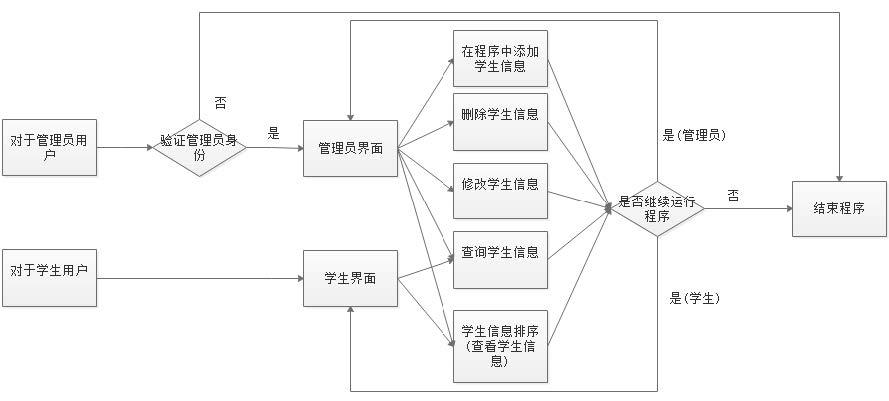
\includegraphics[width=0.6\textwidth]{01WholeStructure.jpg}
		}{\caption{程序整体架构图}\label{fig:WholeStructure}}
	\end{floatrow}
\end{figure}
\subsection{代码文件组成}
该程序代码为标准的QT5 Widgets Application 的工程代码,包含以下几部
分,如\autoref{tab:class}所示:
\begin{table}[!htb]
	\caption[程序的代码组成]{程序的代码组成\label{tab:class}}
	\begin{tabular}{ccc}
		\toprule
		文件名 & 后缀 & 实现的功能 \\
		\midrule
		addstudentwidget & .cpp .h .ui & 增加学生信息界面\\
		adminmenuwidget &.cpp .h .ui &管理员模式菜单界面\\
		adminwidget& .cpp .h .ui &管理员模式窗口界面\\
		delwidget& .cpp .h .ui &删除学生信息界面\\
		findwidget &.cpp .h .ui &查找学生信息界面\\
		mainwidget &.cpp .h .ui &登录主窗口程序界面\\
		sortwidget &.cpp .h .ui &排序(输出)学生信息菜单界面\\
		stumenuwidget &.cpp .h .ui &学生模式菜单界面\\
		stuwidget& .cpp .h .ui &学生模式窗口界面\\
		node &.cpp .h &以链表形式存储信息和功能实现函数\\
		stuinfo &.cpp .h &以类表示学生信息\\
		main& .cpp &主函数\\
		stuinfo &.pro QT5 &工程文件\\
		\bottomrule
	\end{tabular}
\end{table}

\subsection{函数列表}
对addstudentwidget.cpp,包含构造和析构函数,以及返回主菜单按钮的槽
函数on\_returnButton\_clicked、增加学生信息的槽函数on\_addButton\_clicked。\\
对adminwidget.cpp,包含构造和析构函数。\\
对adminmenuwidget.cpp,包含构造和析构函数,以及各个按钮的槽函数。\\
对delwidget.cpp,包含构造和析构函数,以及返回主菜单按钮的槽函数
on\_returnButton\_clicked、删除学生信息的槽函数on\_deletepushButton\_clicked。\\
对findwidget.cpp,包含构造和析构函数,以及返回主菜单按钮的槽函数
on\_returnButton\_clicked、查找学生信息的槽函数on\_pushButton\_clicked。\\
对mainwidget.cpp,包含构造和析构函数。\\
对menuwidget.cpp,包含构造和析构函数,以及登录界面各个按钮的槽函
数。\\
对modifywidget.cpp,包含构造和析构函数,以及返回主菜单按钮的槽函数
on\_returnButton\_clicked、查询修改前学生信息的槽函数on\_searchButton\_clicked,
修改学生信息的槽函数on\_modifypushButton\_clicked。\\
对sortwidget.cpp,包含构造和析构函数,以及返回主菜单按钮的槽函数
on\_returnButton\_clicked、获取学生信息的函数getStuInfo,std::sort 所需的排序
函数cmp\_number 和cmp\_score,排序学生信息的槽函数on\_modifypushButton\_clicked。\\
对stuwidget.cpp,包含构造和析构函数。\\
对stumenuwidget.cpp,包含构造和析构函数,以及各个按钮的槽函数。\\
对stuinfo.cpp, 包含构造和析构函数,以及传递信息的相关函数,在此不表。\\
对Node.cpp, 包含构造函数,从文件获取信息函数InputStudent,删除学生
信息函数DeleteStudent,输出信息到文件函数OutputStudent, 修改学生信息函数
ChangeStudent,查找学生信息函数SearchStudent, 相关函数的声明如下。\\
• void InputStudent();\\
• void DeleteStudent(long long number);\\
• void OutputStudent();\\
• void ChangeStudent(QString name,long long number,QString age,QString gender,\\
long long tel,QString bir,QString address,double score);\\
• bool SearchStudent(QString \&name,long long number,QString \&age,QString \&gender,\\
long long \&tel,QString \&bir,QString \&address,double \&score);\\


%\section{详细设计说明}
%\subsection{插图浮动体}
%在\enquote{nwafuprojrep.cls}模板中,除了可以使用普通的figure浮动体环境
%结合graphicx宏包实现插图排版外,还可以使用floatrow增强浮动体宏包进行浮
%动体排版(适合多图并排、子图排版等)。有关该宏包的使用细节,请在命令行使
%用\enquote{texdoc floatrow}命令查看其使用说明书。例如,可以
%用\autoref{texcode01}排版\autoref{sharefig:a}。

%% 该center环境中的代码为排版示例代码,实际排版中不需要该代码
%\begin{center}
%\begin{langCVOne}[tex][texcode01][\LaTeX{}]{排版单一插图浮动体}
%  \begin{figure}[!htp]
%    \begin{floatrow}
%      \ffigbox[\FBwidth]{
%        \includegraphics[width=0.4\textwidth]{example-image-a}
%      }{\caption{一个插图}\label{sharefig:a}}
%    \end{floatrow}
%  \end{figure}
%\end{langCVOne}
%\end{center}
%
%\begin{figure}[!htp]
%  \begin{floatrow}
%    \ffigbox[\FBwidth]{
%      \includegraphics[width=0.4\textwidth]{example-image-a}
%    }{\caption{一个插图}\label{sharefig:a}}
%  \end{floatrow}
%\end{figure}

%当然,也可以用\autoref{texcode02}排版带有子图的\autoref{trifig}。  

% 该center环境中的代码为排版示例代码,实际排版中不需要该代码
%\begin{center}
%\begin{langCVOne}[tex][texcode02][\LaTeX{}]{排版单一插图浮动体}
%\begin{figure}[!htp]
%  \ffigbox[\textwidth]%
%  {%
%    \begin{subfloatrow}[2]%\useFCwidth
%      \ffigbox[\FBwidth]{
%        \includegraphics[width=0.3\textwidth]{example-image-a}
%      }{\caption{子题注1}\label{trifig:a}}
%      \ffigbox[\FBwidth]{
%        \includegraphics[width=0.3\textwidth]{example-image-b}
%      }{\caption{子题注2}\label{trifig:b}}
%    \end{subfloatrow}    
%    \begin{subfloatrow}[2]%\useFCwidth      
%      \ffigbox[\FBwidth]{
%        \includegraphics[width=0.3\textwidth]{example-image-c}
%      }{\caption{子题注3}\label{trifig:c}}
%      \ffigbox[\FBwidth]{
%        \includegraphics[width=0.3\textwidth]{example-image}
%      }{\caption{子题注4}\label{trifig:d}}
%    \end{subfloatrow}
%  }{\caption{四个子图}\label{trifig}}
%\end{figure}
%\end{langCVOne}
%\end{center}
\section{详细设计说明}
\subsection{增加学生信息函数}
这是一个无参函数,实现新增一位学生信息的功能,新的学生信息节点默
认添加到链表尾部。
算法:定义节点指针p,指向第一个学生信息节点p=pHead->pNext,通过
while 循环将其指向尾节点,读入学生信息并将其写入新建节点pt 中,p->pNext
指向新节点pt,pt->pNext 为NULL,添加完成。
流程图如\autoref{fig:addstudent}:
\begin{figure}[!htp]
	\begin{floatrow}
		\ffigbox[\FBwidth]{
			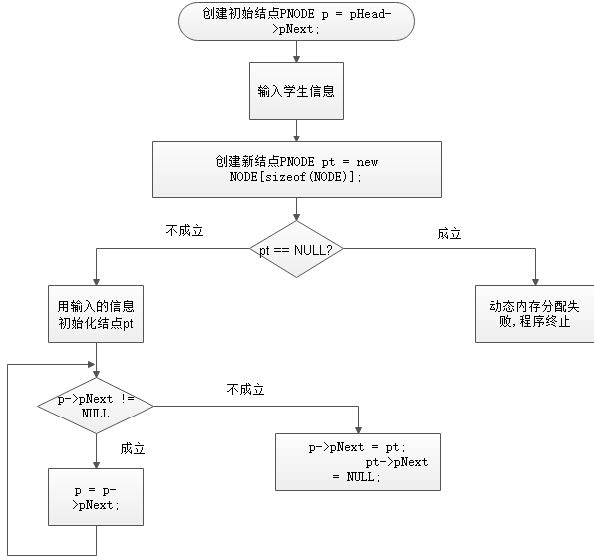
\includegraphics[width=0.6\textwidth]{02addstudent.jpg}
		}{\caption{增加学生信息函数流程图}\label{fig:addstudent}}
	\end{floatrow}
\end{figure}

\subsection{输入学生信息函数}
Void InputStudent() 这是一个无参函数,实现将文件中存储的学生信息读入
到程序中。
算法:先声明一个头节点pHead,并创建一个指向头节点的指针pTail,每
输入一个学生的信息就声明一个新节点pNew 来存储信息,把pNew 挂到老节
点后面,同时移动pTail 到pNew 上并使pTail->pNext = NULL。
流程图如\autoref{fig:inputstudent}:
\begin{figure}[!htp]
	\begin{floatrow}
		\ffigbox[\FBwidth]{
			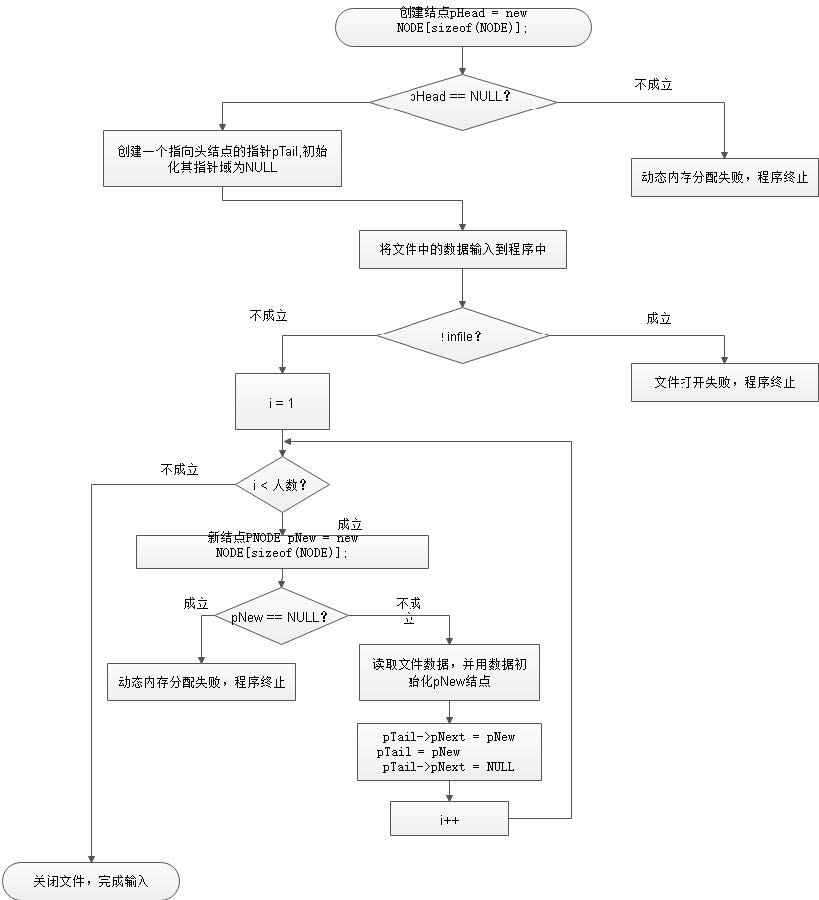
\includegraphics[width=0.6\textwidth]{03inputstudent.jpg}
		}{\caption{输入学生信息函数流程图}\label{fig:inputstudent}}
	\end{floatrow}
\end{figure}

\subsection{输出学生信息函数}
这是一个无参函数,负责对链表中全部学生信息的输出。
算法:先将p 节点的指针指向第一个节点,将p 节点(即第一个节点)的
数据输出。然后再将p 节点的指针指向下一个节点,即p = p -> pNext,再次将
p 节点的数据输出。重复执行此步骤直到p 指针指向NULL 为止。
流程图如\autoref{fig:outputstudent}:
\begin{figure}[!htp]
	\begin{floatrow}
		\ffigbox[\FBwidth]{
			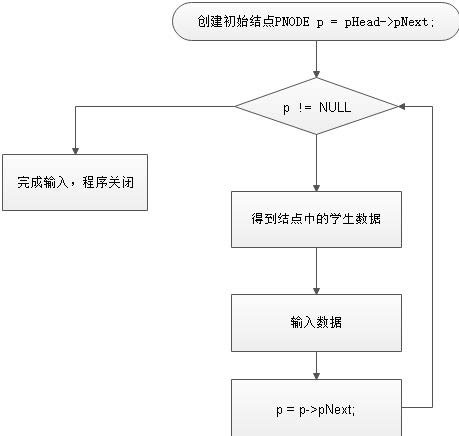
\includegraphics[width=0.6\textwidth]{04outputstudent.jpg}
		}{\caption{输出学生信息函数流程图}\label{fig:outputstudent}}
	\end{floatrow}
\end{figure}

\subsection{删除学生信息函数}


\section{temp}
\begin{figure}[!htp]
  \ffigbox[\textwidth]%
  {%
    \begin{subfloatrow}[2]%\useFCwidth
      \ffigbox[\FBwidth]{
        \includegraphics[width=0.25\textwidth]{example-image-a}
      }{\caption{子题注1}\label{trifig:a}}
      \ffigbox[\FBwidth]{
        \includegraphics[width=0.25\textwidth]{example-image-b}
        
      }{\caption{子题注2}\label{trifig:b}}
    \end{subfloatrow}    
    \begin{subfloatrow}[2]%\useFCwidth      
      \ffigbox[\FBwidth]{
        \includegraphics[width=0.25\textwidth]{example-image-c}
      }{\caption{子题注3}\label{trifig:c}}
      \ffigbox[\FBwidth]{
        \includegraphics[width=0.25\textwidth]{example-image}
      }{\caption{子题注4}\label{trifig:d}}
    \end{subfloatrow}
  }{\caption{四个子图}\label{trifig}}
\end{figure}

在模板中,已为插图设置
了{{./figs/}、{./figure/}、{./figures/}、{./image/}、{./images/}、
  {./graphics/}、{./graphic/}、{./pictures/}、{./picture/}}相对路径,可
以在当前工作路径中任意一个这样命名的文件夹,以存放需要的插图文件。

\subsection{表格浮动体}
如果需要插入一个简单的表格,可以仅使用{table}和{tabular}环境实现,如%
\autoref{tab:city}。

\emph{注意:}科技文档中的表格需要采用\emph{三线表}。

\begin{table}[!htb]
  \caption[城市人口]{城市人口数量排名 (source: Wikipedia)\label{tab:city}}
  \begin{tabular}{lr}
    \toprule
    城市 & 人口 \\
    \midrule
    Mexico City & 20,116,842\\
    Shanghai & 19,210,000\\
    Peking & 15,796,450\\
    Istanbul & 14,160,467\\
    \bottomrule
  \end{tabular}
\end{table}

如果多个表格布局较为复杂,可以使用floatrow宏包实现排版。如用\autoref{texcodetab}可编制\autoref{tab:testsample}和\autoref{tab:city2}所示的横向并排表格。


% 该center环境中的代码为排版示例代码,实际排版中不需要该代码
\begin{center}
  \begin{langCVOne}[tex][texcodetab][\LaTeX{}]{表格排版}
    % 横向排版两个表格
    \begin{table}[!htp]
      \begin{floatrow}
        \ttabbox[\FBwidth]
        {
          \begin{tabular}{ccl}
            \toprule
            序号 & 测试用例 & \multicolumn{1}{c}{测试目的}\\
            \midrule
            1 & a & 小写字母到大写字母转换\\
            2 & A & 大写字母到小写字母转换\\
            3 & @ & 非字母字符测试\\
            4 & 2 & 非字母其它字符\\
            \bottomrule
          \end{tabular}      
        }{\caption{字母大小写转换测试用例表}\label{tab:testsample}}
        \ttabbox[\FBwidth]
        {
          \begin{tabular}{lr}
            \toprule
            城市 & 人口 \\
            \midrule
            Mexico City & 20,116,842\\
            Shanghai & 19,210,000\\
            Peking & 15,796,450\\
            Istanbul & 14,160,467\\
            \bottomrule
          \end{tabular}      
        }{\caption{城市人口数量排名}\label{tab:city2}}
      \end{floatrow}
    \end{table}
  \end{langCVOne}
\end{center}

% 横向排版两个表格
\begin{table}[!htp]
  \begin{floatrow}
    \ttabbox[\FBwidth]
    {
      \begin{tabular}{ccl}
        \toprule
        序号 & 测试用例 & \multicolumn{1}{c}{测试目的}\\
        \midrule
        1 & a & 小写字母到大写字母转换\\
        2 & A & 大写字母到小写字母转换\\
        3 & @ & 非字母字符测试\\
        4 & 2 & 非字母其它字符\\
        \bottomrule
      \end{tabular}      
    }{\caption{字母大小写转换测试用例表}\label{tab:testsample}}
    \ttabbox[\FBwidth]
    {
      \begin{tabular}{lr}
        \toprule
        城市 & 人口 \\
        \midrule
        Mexico City & 20,116,842\\
        Shanghai & 19,210,000\\
        Peking & 15,796,450\\
        Istanbul & 14,160,467\\
        \bottomrule
      \end{tabular}      
    }{\caption{城市人口数量排名}\label{tab:city2}}
  \end{floatrow}
\end{table}

% \begin{table}[!htp]
%   \ttabbox[\FBwidth]{
%     \begin{tabular}{ccl}
%       \toprule
%       序号 & 测试用例 & \multicolumn{1}{c}{测试目的}\\
%       \midrule
%       1 & a & 小写字母到大写字母转换\\
%       2 & A & 大写字母到小写字母转换\\
%       3 & @ & 非字母字符测试\\
%       4 & 2 & 非字母其它字符\\
%       \bottomrule      
%     \end{tabular}
%   }{\caption{字母大小写转换测试用例表}\label{tab:testsample}}
% \end{table}

如果表格内容很多,导致无法放在一页内的话,需要用{longtable} 或{longtabu} 进行分页。
\autoref{tab:performance}是一个长表格的例子。

% 定义表中用到的的宏,以简化表格代码并为后续修改提供统一接口
\def\tabcaption{实验数据,这个题注十分的长,注意这在索引中的处理方式,还有 \cs{caption} 后面的双反斜杠}
\def\tabheadrow{
  \multirow{2}{*}{测试程序} & \multicolumn{1}{c}{正常运行} &
   \multicolumn{1}{c}{同步} & \multicolumn{1}{c}{检查点} &
   \multicolumn{1}{c}{卷回恢复} & \multicolumn{1}{c}{进程迁移} &
   \multicolumn{1}{c}{检查点} \\
   & \multicolumn{1}{c}{时间(s)} & \multicolumn{1}{c}{时间(s)} &
   \multicolumn{1}{c}{时间(s)} & \multicolumn{1}{c}{时间(s)} &
   \multicolumn{1}{c}{时间(s)} & \multicolumn{1}{c}{文件(KB)} \\
 }

% 定义跨页表续表表题
\def\ctntabcap{
   \multicolumn{7}{c}{\small\heiti{}续表~\thetable\hskip1em 实验测试数据}  
 }
 % 定义跨页表命令集合
\def\ctntabcmd{
   \\\ctntabcap\\
   \toprule
   \tabheadrow
   \midrule
   \endhead
   \midrule
   \multicolumn{7}{r}{续下页}\\
   \endfoot
   \endlastfoot  
 } 
 
 
\begin{longtable}[c]{c*{6}{r}}
        \caption[实验数据]{实验测试数据}\label{tab:performance}\\
        \toprule
        \tabheadrow
        \midrule
        \endfirsthead
        \ctntabcmd
        CG.A.2 & 23.05 & 0.002 & 0.116 & 0.035 & 0.589 & 32491 \\
        CG.A.4 & 15.06 & 0.003 & 0.067 & 0.021 & 0.351 & 18211 \\
        CG.A.8 & 13.38 & 0.004 & 0.072 & 0.023 & 0.210 & 9890 \\
        CG.B.2 & 867.45 & 0.002 & 0.864 & 0.232 & 3.256 & 228562 \\
        CG.B.4 & 501.61 & 0.003 & 0.438 & 0.136 & 2.075 & 123862 \\
        CG.B.8 & 384.65 & 0.004 & 0.457 & 0.108 & 1.235 & 63777 \\
        MG.A.2 & 112.27 & 0.002 & 0.846 & 0.237 & 3.930 & 236473 \\
        MG.A.4 & 59.84 & 0.003 & 0.442 & 0.128 & 2.070 & 123875 \\
        MG.A.8 & 31.38 & 0.003 & 0.476 & 0.114 & 1.041 & 60627 \\
        MG.B.2 & 526.28 & 0.002 & 0.821 & 0.238 & 4.176 & 236635 \\
        MG.B.4 & 280.11 & 0.003 & 0.432 & 0.130 & 1.706 & 123793 \\
        MG.B.8 & 148.29 & 0.003 & 0.442 & 0.116 & 0.893 & 60600 \\
        LU.A.2 & 2116.54 & 0.002 & 0.110 & 0.030 & 0.532 & 28754 \\
        LU.A.4 & 1102.50 & 0.002 & 0.069 & 0.017 & 0.255 & 14915 \\
        LU.A.8 & 574.47 & 0.003 & 0.067 & 0.016 & 0.192 & 8655 \\
        LU.B.2 & 9712.87 & 0.002 & 0.357 & 0.104 & 1.734 & 101975 \\
        LU.B.4 & 4757.80 & 0.003 & 0.190 & 0.056 & 0.808 & 53522 \\
        LU.B.8 & 2444.05 & 0.004 & 0.222 & 0.057 & 0.548 & 30134 \\
        CG.B.2 & 867.45 & 0.002 & 0.864 & 0.232 & 3.256 & 228562 \\
        CG.B.4 & 501.61 & 0.003 & 0.438 & 0.136 & 2.075 & 123862 \\
        CG.B.8 & 384.65 & 0.004 & 0.457 & 0.108 & 1.235 & 63777 \\
        MG.A.2 & 112.27 & 0.002 & 0.846 & 0.237 & 3.930 & 236473 \\
        MG.A.4 & 59.84 & 0.003 & 0.442 & 0.128 & 2.070 & 123875 \\
        MG.A.8 & 31.38 & 0.003 & 0.476 & 0.114 & 1.041 & 60627 \\
        MG.B.2 & 526.28 & 0.002 & 0.821 & 0.238 & 4.176 & 236635 \\
        MG.B.4 & 280.11 & 0.003 & 0.432 & 0.130 & 1.706 & 123793 \\
        MG.B.8 & 148.29 & 0.003 & 0.442 & 0.116 & 0.893 & 60600 \\
        LU.A.2 & 2116.54 & 0.002 & 0.110 & 0.030 & 0.532 & 28754 \\
        LU.A.4 & 1102.50 & 0.002 & 0.069 & 0.017 & 0.255 & 14915 \\
        LU.A.8 & 574.47 & 0.003 & 0.067 & 0.016 & 0.192 & 8655 \\
        LU.B.2 & 9712.87 & 0.002 & 0.357 & 0.104 & 1.734 & 101975 \\
        LU.B.4 & 4757.80 & 0.003 & 0.190 & 0.056 & 0.808 & 53522 \\
        LU.B.8 & 2444.05 & 0.004 & 0.222 & 0.057 & 0.548 & 30134 \\
        EP.A.2 & 123.81 & 0.002 & 0.010 & 0.003 & 0.074 & 1834 \\
        EP.A.4 & 61.92 & 0.003 & 0.011 & 0.004 & 0.073 & 1743 \\
        EP.A.8 & 31.06 & 0.004 & 0.017 & 0.005 & 0.073 & 1661 \\
        EP.B.2 & 495.49 & 0.001 & 0.009 & 0.003 & 0.196 & 2011 \\
        EP.B.4 & 247.69 & 0.002 & 0.012 & 0.004 & 0.122 & 1663 \\
        EP.B.8 & 126.74 & 0.003 & 0.017 & 0.005 & 0.083 & 1656 \\
        \bottomrule
   \end{longtable}

\subsection{插图标注}
在\enquote{nwafuprojrep.cls}模板中,可能通过引入了改自tikz-imagelabels宏包
的tikz-imglabels宏包,利用TikZ为插图进行标注。该宏包的使用细节与
tikz-imagelabels完全一致,请在命令行使用\enquote{texdoc tikz-imagelabels}命令
查看其使用说明书。\autoref{texcode03}用于实现\autoref{fig:annot}所示的插图标注。

% 该center环境中的代码为排版示例代码,实际排版中不需要该代码
\begin{center}
\begin{langCVOne}[tex][texcode03][\LaTeX{}]{插图标注代码}
\begin{figure}[!htp]
  \centering
    \begin{annotationimage}{width=0.8\textwidth}{figs/01reviewicons01}
      % 绘制外观设置按钮分组示意下划线
      \draw[thick,blue] (0.86,0.26) -- (1.0,0.26);
      % 添加各图标标注
      \foreach \ann/\xpos in
      {
        {附\\注\\工\\具}/0.02, {高\\亮\\工\\具}/0.07,
        {下\\划\\线\\工\\具}/0.126, {删\\除\\线\\工\\具}/0.18,
        {删\\除\\线\\并\\插\\入\\附\\注\\工\\具}/0.229, {插\\入\\文\\本\\工\\具}/0.283,
        {文\\本\\工\\具}/0.346, {文\\本\\框\\工\\具}/0.40,
        {铅\\笔\\绘\\图\\工\\具}/0.45, {铅\\笔\\擦\\工\\具}/0.51,
        {图\\章\\工\\具}/0.56, {附\\加\\文\\件\\工\\具}/0.63,
        {绘\\图\\工\\具}/0.7, {保\\持\\选\\择\\工\\具}/0.79,
        {注\\释\\外\\观\\设\\置}/0.93
      }
      {
        \draw[annotation below = {{\ann} at \xpos}] to (\xpos,0.48);
      }
    \end{annotationimage}
    \caption{插图标注}\label{fig:annot}
  \end{figure}
\end{langCVOne}
\end{center}

% 图像标注
\begin{figure}[!htp]
  \centering
  \begin{annotationimage}{width=0.8\textwidth}{figs/01reviewicons01}
    % 绘制外观设置按钮分组示意下划线
    \draw[thick,blue] (0.86,0.26) -- (1.0,0.26);
    % 添加各图标标注
    \foreach \ann/\xpos in
    {
      {附\\注\\工\\具}/0.02, {高\\亮\\工\\具}/0.07,
      {下\\划\\线\\工\\具}/0.126, {删\\除\\线\\工\\具}/0.18,
      {删\\除\\线\\并\\插\\入\\附\\注\\工\\具}/0.229, {插\\入\\文\\本\\工\\具}/0.283,
      {文\\本\\工\\具}/0.346, {文\\本\\框\\工\\具}/0.40,
      {铅\\笔\\绘\\图\\工\\具}/0.45, {铅\\笔\\擦\\工\\具}/0.51,
      {图\\章\\工\\具}/0.56, {附\\加\\文\\件\\工\\具}/0.63,
      {绘\\图\\工\\具}/0.7, {保\\持\\选\\择\\工\\具}/0.79,
      {注\\释\\外\\观\\设\\置}/0.93
    }
    {
      \draw[annotation below = {{\ann} at \xpos}] to (\xpos,0.48);
    }
  \end{annotationimage}
  \caption{插图标注}\label{fig:annot}
\end{figure}

\subsection{流程图}
在\enquote{nwafuprojrep.cls}模板中,可能引入了自己开发
的tikz-flowchart宏包进行流程图的绘制。请
在\github{}查看%
\href{https://github.com/registor/tikz-flowchart}{tikz-flowchart宏包}的
使用说明书。

在绘制流程图时,可以先用纸和笔绘制草稿,然后根据草稿布置各个结点,再
连接流程线。这样,可以做到心中有数,绘制较为方便。

\autoref{subfig:draft}是一个流程图草稿。根据该草稿,基于tikz-flowchart宏包,
用\autoref{texcode04}可绘制\autoref{subfig:tikz}所示的流程图。

% 该center环境中的代码为排版示例代码,实际排版中不需要该代码
\begin{center}
  \begin{langCVOne}[tex][texcode04][\LaTeX{}]{绘制流程图}
    % 流程图绘制属性设置
    \flowchartset{
      proc fill color = orange!10, % 顺序处理框填充颜色(默认取白色)
      test fill color = green!30, % 判断框填充颜色(默认取白色)
      io fill color = blue!30, % 输入/输出框填充颜色(默认取白色)
      term fill color = red!30, % 开始/结束框填充颜色(默认取白色)
    }
    % 绘制流程图
    \begin{tikzpicture}[scale=0.53,transform shape,]
      % 布置结点单元
      \node [term] (st) {开始};
      \node [proc, text width = 5em, join] (p1) {int divisor};       
      \node [test, join] (t1) {n <= 1};
      \node [proc, text width = 5em] (p2) {divisor = 2};
      \node [test, text width = 10em, join] (t2) {divisor * divisor <= n};
      \node [test, text width = 8em] (t3) {n \% divisor == 0};
      \node [proc, text width = 5em] (p3) {divisor++};
      \node [term, below = 1.6 of p3] (end) {结束};
      \node [proc, text width = 4em, left = 4.8 of t2] (p4) {return 0};
      \node [proc, text width = 4em, right = 3.5 of p3] (p5) {return 0};
      \node [proc, text width = 4em, right = 5.8 of t3] (p6) {return 1};

      % 布置用于连接的坐标结点,同时为其布置调试标记点。
      \node [coord] (c1) at ($(p2.south)!0.5!(t2.north)$)  {}; \cmark{1}
      \node [coord, below = 0.25 of p3] (c2)  {}; \cmark{2}
      \node [coord, above = 0.5 of end] (c3) {};  \cmark{3}
      \node [coord, left = 0.5 of t2] (ct) {};  \cmark{t}
      \node [coord] (c4) at (c3 -| p5)  {}; \cmark{4}
      \node [coord] (c5) at (c2 -| ct)  {}; \cmark{5}
        
      % 判断框连线,每次绘制时,先绘制一个带有一个固定
      % 位置标注的路径(path),然后再绘制箭头本身(arrow)。
      \path (t1.south) -- node [near start, right] {$N$} (p2.north);
      \draw [norm] (t1.south) -- (p2.north);
      \path (t1.west) -| node [near start, above] {$Y$} (p4.north);
      \draw [norm] (t1.west) -| (p4.north);
      
      \path (t2.south) -- node [near start, right] {$Y$} (t3.north);
      \draw [norm] (t2.south) -- (t3.north);
      \path (t2.east) -| node [near start, above] {$N$} (p6.north);
      \draw [norm] (t2.east) -| (p6.north);
      
      \path (t3.south) -- node [near start, right] {$N$} (p3.north);
      \draw [norm] (t3.south) -- (p3.north);
      \path (t3.east) -| node [near start, above] {$Y$} (p5.north);
      \draw [norm] (t3.east) -| (p5.north);

      % 其它连线
      \draw [norm](p3.south) |- (c5) |- (c1);
      \draw [norm](p4.south) |- (c3);
      \draw [norm](p4.south) |- (c3) -- (end);
      \draw [norm](p5.south) -- (c4);
      \draw [norm](p6.south) |- (c3);
      \draw [norm](p6.south) |- (c3) -- (end);
    \end{tikzpicture}
  \end{langCVOne}
\end{center}

% 流程图绘制属性设置
\flowchartset{
  proc fill color = orange!10, % 顺序处理框填充颜色(默认取白色)
  test fill color = green!30, % 判断框填充颜色(默认取白色)
  io fill color = blue!30, % 输入/输出框填充颜色(默认取白色)
  term fill color = red!30, % 开始/结束框填充颜色(默认取白色)
}

\begin{figure}[!htp]
  \ffigbox[\textwidth]%
  {%
    \begin{subfloatrow}[2]%\useFCwidth
      \ffigbox[\FBwidth]{
        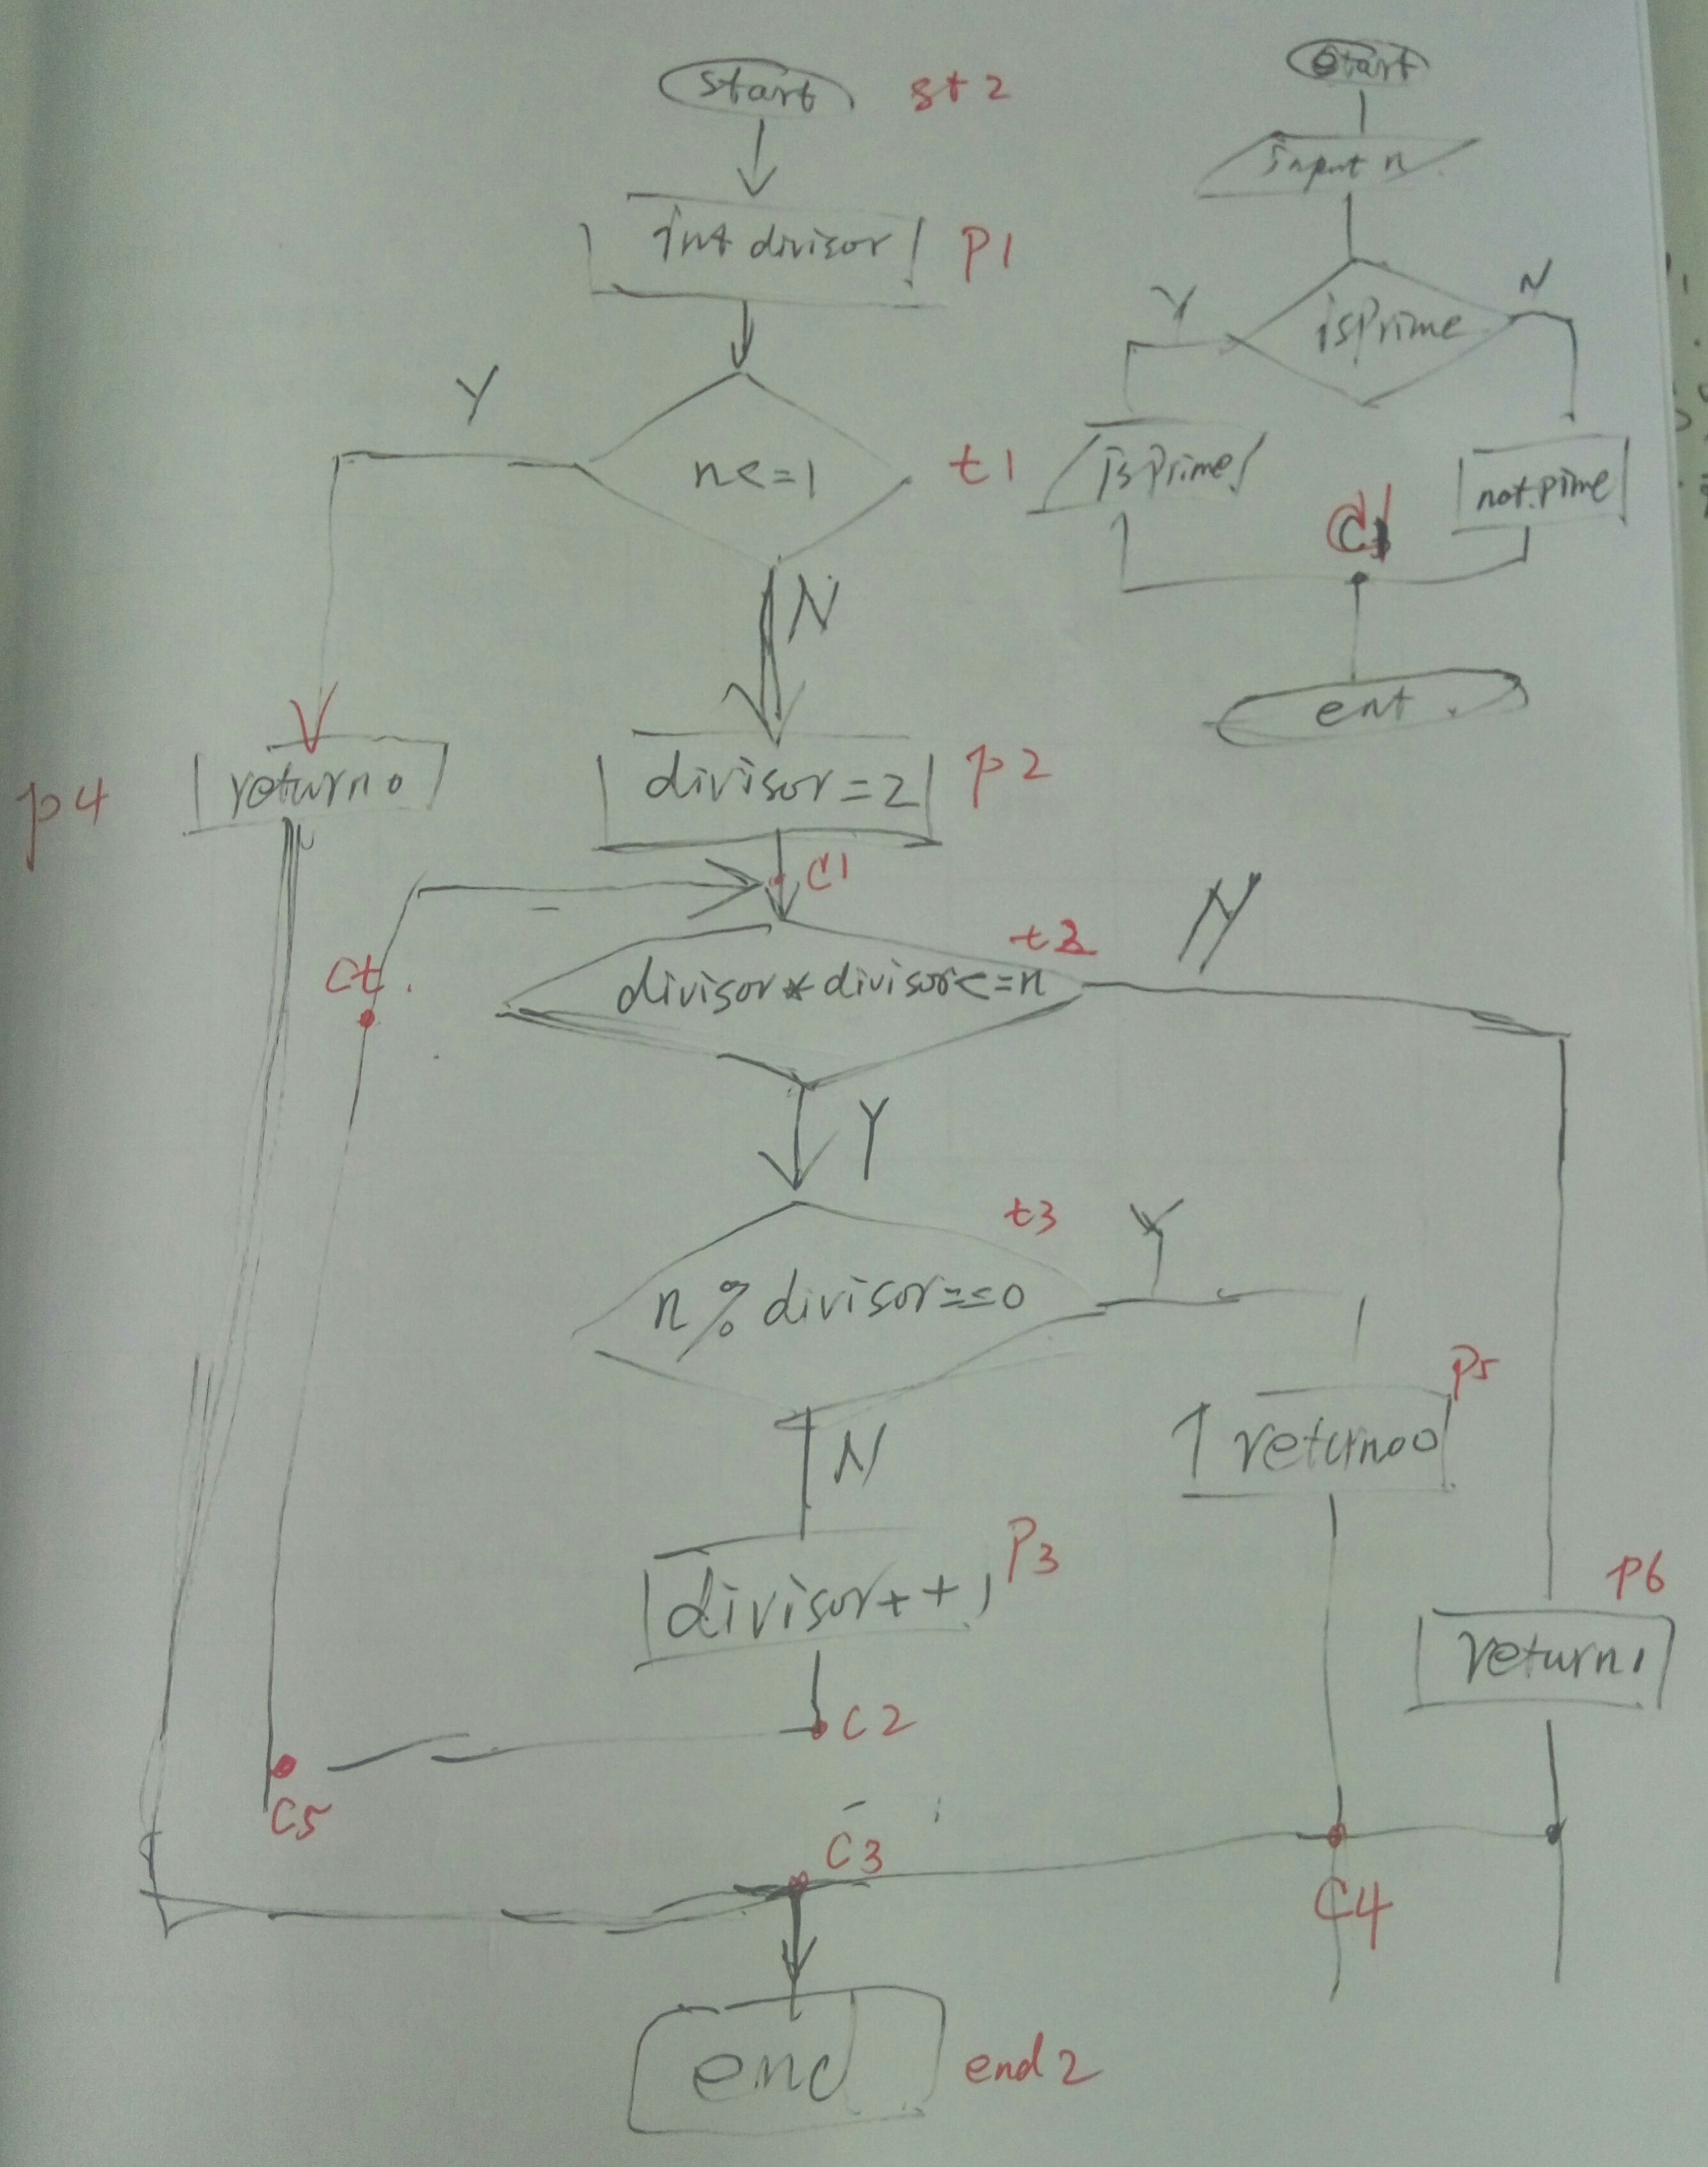
\includegraphics[width=0.35\textwidth]{02gcd}
      }{\caption{草图}\label{subfig:draft}}
      \ffigbox[\FBwidth]{
        \begin{tikzpicture}[scale=0.53,transform shape,]
          % 布置结点单元
          \node [term] (st) {开始};
          \node [proc, text width = 5em, join] (p1) {int divisor};       
          \node [test, join] (t1) {n <= 1};
          \node [proc, text width = 5em] (p2) {divisor = 2};
          \node [test, text width = 10em, join] (t2) {divisor * divisor <= n};
          \node [test, text width = 8em] (t3) {n \% divisor == 0};
          \node [proc, text width = 5em] (p3) {divisor++};
          \node [term, below = 1.6 of p3] (end) {结束};
          \node [proc, text width = 4em, left = 4.8 of t2] (p4) {return 0};
          \node [proc, text width = 4em, right = 3.5 of p3] (p5) {return 0};
          \node [proc, text width = 4em, right = 5.8 of t3] (p6) {return 1};

          % 布置用于连接的坐标结点,同时为其布置调试标记点。
          \node [coord] (c1) at ($(p2.south)!0.5!(t2.north)$)  {}; \cmark{1}
          \node [coord, below = 0.25 of p3] (c2)  {}; \cmark{2}
          \node [coord, above = 0.5 of end] (c3) {};  \cmark{3}
          \node [coord, left = 0.5 of t2] (ct) {};  \cmark{t}
          \node [coord] (c4) at (c3 -| p5)  {}; \cmark{4}
          \node [coord] (c5) at (c2 -| ct)  {}; \cmark{5}
        
          % 判断框连线,每次绘制时,先绘制一个带有一个固定
          % 位置标注的路径(path),然后再绘制箭头本身(arrow)。
          \path (t1.south) -- node [near start, right] {$N$} (p2.north);
          \draw [norm] (t1.south) -- (p2.north);
          \path (t1.west) -| node [near start, above] {$Y$} (p4.north);
          \draw [norm] (t1.west) -| (p4.north);
        
          \path (t2.south) -- node [near start, right] {$Y$} (t3.north);
          \draw [norm] (t2.south) -- (t3.north);
          \path (t2.east) -| node [near start, above] {$N$} (p6.north);
          \draw [norm] (t2.east) -| (p6.north);
        
          \path (t3.south) -- node [near start, right] {$N$} (p3.north);
          \draw [norm] (t3.south) -- (p3.north);
          \path (t3.east) -| node [near start, above] {$Y$} (p5.north);
          \draw [norm] (t3.east) -| (p5.north);

          % 其它连线
          \draw [norm](p3.south) |- (c5) |- (c1);
          \draw [norm](p4.south) |- (c3);
          \draw [norm](p4.south) |- (c3) -- (end);
          \draw [norm](p5.south) -- (c4);
          \draw [norm](p6.south) |- (c3);
          \draw [norm](p6.south) |- (c3) -- (end);
        \end{tikzpicture}
      }{\caption{TiKZ绘制图}\label{subfig:tikz}}
    \end{subfloatrow}
  }{\caption{用TiKZ绘制流程图}\label{fig:flowcharttikzdraw}}
\end{figure}

\subsection{UML图}
可以使用\enquote{pgf-umlcd}宏包实现UML图的绘制,在命令行
使用\enquote{texdoc pgf-umlcd}查看该宏包的使用说明书。

但由于TeXLive收集的pgf-umlcd宏包不能很好的处理中文类名,因此请使用模板
提供的pgf-umlcd宏包排版UML图。

\autoref{fig:uml}是使用\enquote{pgf-umlcd}宏包绘制的UML图。
\begin{figure}[!hpt]
  \centering
  \begin{tikzpicture}[font=\small]
    \tikzset{ coord/.style={coordinate} }    
    \begin{class}[fill=red!25, text width=7em]{动物类CAnimal}{0, 0}
      \attribute{-name[32]:char}
      \attribute{-age:int}
      \attribute{-weight:int}
      \operation{+show():void}
    \end{class}

    \begin{class}[fill=green!25, text width=5em]{马CHorse}{-5, -4.5}
      \inherit{动物类CAnimal}
      \attribute{-power:int}
      \operation{+show():void}
      \operation{+talk():void}
    \end{class}
      
    \begin{class}[fill=green!25, text width=5em]{鸟CBird}{0, -4.5}
      \inherit{动物类CAnimal}
      \attribute{-wingSpan:int}
      \operation{+show():void}
      \operation{+talk():void}
    \end{class}
      
    \begin{class}[fill=green!25, text width=5em]{牛CBull}{5, -4.5}
      \inherit{动物类CAnimal}
      \attribute{-power:int}
      \operation{+show():void}
      \operation{+talk():void}
    \end{class}

    \begin{class}[fill=blue!25, text width=6em]{飞马CPegasus}{-2.5, -8}
      \inherit{马CHorse}
      \inherit{鸟CBird}
      \operation{+show():void}
      \operation{+talk():void}
    \end{class}           
  \end{tikzpicture}  
  \caption{用\enquote{pgf-umlcd}宏包绘制UML图}\label{fig:uml}
\end{figure}

\subsection{代码排版}
在\enquote{nwafuprojrep.cls}模板中,可以引入了自己开发的boxie.sty宏包
进行代码排版。本文档\autoref{secboxiety}中有基本使用样例,详情请在\github{}查看
\href{https://github.com/registor/boxiesty}{boxie宏包}
的使用说明书。

\subsection{列表环境}
在\enquote{nwafuprojrep.cls}模板中,基于enumitem宏包分别对itemize、
enumerate和description三个环境的各个距离参数进行了修正,以使其排版结果
符合中文习惯的首先缩进格式。
\subsubsection{itemize环境}
\begin{itemize}
\item 床前明月光,床前明月光,床前明月光,床前明月光,床前明月光,床前明月光,床前明月光。
\item 疑是地上霜,疑是地上霜,疑是地上霜,疑是地上霜,疑是地上霜,疑是地上霜,疑是地上霜。
\item 举头望明月,举头望明月,举头望明月,举头望明月,举头望明月,举头望明月,举头望明月。
\item 低头思故乡,低头思故乡,低头思故乡,低头思故乡,低头思故乡,低头思故乡,低头思故乡。
\end{itemize}
\subsubsection{enumerate环境}
\begin{enumerate}
\item 床前明月光,床前明月光,床前明月光,床前明月光,床前明月光,床前明月光,床前明月光。
\item 疑是地上霜,疑是地上霜,疑是地上霜,疑是地上霜,疑是地上霜,疑是地上霜,疑是地上霜。
\item 举头望明月,举头望明月,举头望明月,举头望明月,举头望明月,举头望明月,举头望明月。
\item 低头思故乡,低头思故乡,低头思故乡,低头思故乡,低头思故乡,低头思故乡,低头思故乡。
\end{enumerate}
\subsubsection{description环境}
\begin{description}
\item[床前明月光],床前明月光,床前明月光,床前明月光,床前明月光,床前明月光,床前明月光。
\item[疑是地上霜],疑是地上霜,疑是地上霜,疑是地上霜,疑是地上霜,疑是地上霜,疑是地上霜。
\item[举头望明月],举头望明月,举头望明月,举头望明月,举头望明月,举头望明月,举头望明月。
\item[低头思故乡],低头思故乡,低头思故乡,低头思故乡,低头思故乡,低头思故乡,低头思故乡。
\end{description}

\subsection{\enquote{emph}强调字体}
在\enquote{nwafuprojrep.cls}模板中,重定义强调字体,将默认强调字体
是italic,中文用楷体代替操作更换为加粗操作,用加粗后的字体表示强调。
\subsection{文本框盒子}
文本框盒子继承于自己开发的boxie宏包,其使用细节请在\github{}查看
\href{https://github.com/registor/boxiesty}{boxie宏包}的使用说明书。
同时,在该宏包的基础上,为boxie宏包添加加了摘自于
\href{https://github.com/WisdomFusion/latex-templates/tree/master/progartcn}{progartcn
  论文模板}的\enquote{标题}、\enquote{注意}、\enquote{重要}、
\enquote{技巧}和\enquote{警告}文本框环境代码\footnote{本节示例摘自于
  该模板中的tutorial-sample.tex文件}。
\subsubsection{\enquote{标题}文本框}
标题文本框环境的使用格式为:

\verb|\begin{titledBox}{<title>} <content> \end{titledBox}|

\begin{titledBox}{HTTP/Console 内核}
  HTTP 内核继承自 \verb|Illuminate\Foundation\Http\Kernel| 类,该类定义了一个 \verb|bootstrappers| 数组,这个数组中的类在请求被执行前运行,这些 \verb|bootstrappers| 配置了错误处理、日志、检测应用环境以及其它在请求被处理前需要执行的任务。
\end{titledBox}
\subsubsection{\enquote{注意}文本框}
注意文本框环境的使用格式为:

\verb|\begin{noteBox} <content> \end{noteBox}|

\begin{noteBox}
  HTTP 内核继承自 \verb|Illuminate\Foundation\Http\Kernel| 类,该类定义了一个 \verb|bootstrappers| 数组,这个数组中的类在请求被执行前运行,这些 \verb|bootstrappers| 配置了错误处理、日志、检测应用环境以及其它在请求被处理前需要执行的任务。
\end{noteBox}

\subsubsection{\enquote{重要}文本框}
重要文本框环境的使用格式为:

\verb|\begin{importantBox} <content> \end{importantBox}|

\begin{importantBox}
  HTTP 内核继承自 \verb|Illuminate\Foundation\Http\Kernel| 类,该类定义了一个 \verb|bootstrappers| 数组,这个数组中的类在请求被执行前运行,这些 \verb|bootstrappers| 配置了错误处理、日志、检测应用环境以及其它在请求被处理前需要执行的任务。
\end{importantBox}
\subsubsection{\enquote{技巧}文本框}
技巧文本框环境的使用格式为:

\verb|\begin{tipBox} <content> \end{tipBox}|

\begin{tipBox}
  HTTP 内核继承自 \verb|Illuminate\Foundation\Http\Kernel| 类,该类定义了一个 \verb|bootstrappers| 数组,这个数组中的类在请求被执行前运行,这些 \verb|bootstrappers| 配置了错误处理、日志、检测应用环境以及其它在请求被处理前需要执行的任务。
\end{tipBox}
\subsubsection{\enquote{警告}文本框}
警告文本框环境的使用格式为:

\verb|\begin{warningBox} <content> \end{warningBox}|

\begin{warningBox}
  HTTP 内核继承自 \verb|Illuminate\Foundation\Http\Kernel| 类,该类定义了一个 \verb|bootstrappers| 数组,这个数组中的类在请求被执行前运行,这些 \verb|bootstrappers| 配置了错误处理、日志、检测应用环境以及其它在请求被处理前需要执行的任务。
\end{warningBox}

\subsection{交叉引用}
在技术文档中,图、表、公式等必须使用\emph{交叉引用},
在\enquote{nwafuprojrep.cls}模板中,交叉引用
用\verb|\autoref|命令实现引用,并对图、表、节、小节、公式、代码等引用
标记字/词进行了设置。如对一个标签为\enquote{fig:01}的图使用
\verb|\autoref{fig:01}|便可以得到\enquote{图 XX}的结果,用
\verb|\autoref{texcode01}|就可以得到\enquote{代码 XX}的结果。

\subsection{参考文献}
参考文献采用GB/T7714-2015标准的顺序编码制,使用biber+biblatex方式实现,
样式控制选择\enquote{biblatex-gb7714-2015}宏包的顺序编码制
(gb7714-2015)样式,如\autoref{texcode06}:

\begin{center}
  \begin{langCVOne}[tex][texcode06][\LaTeX{}]{引用参考文献}
    % 引用参考文献
    详见文献\cite{Peebles2001-100-100}\parencite{Babu2014--}
    另见文献\cite[49]{于潇2012-1518-1523}\parencite[106]{Babu2014--}
  \end{langCVOne}
\end{center}

能够生成如下引用结果:

% 引用参考文献
详见文献\cite{Peebles2001-100-100}\parencite{Babu2014--}
另见文献\cite[49]{于潇2012-1518-1523}\parencite[106]{Babu2014--}

\subsection{已载入的宏包}
在\enquote{nwafuprojrep.cls}模板中,已引入的宏包有:
\verb|etoolbox|、\verb|unicode-math|、\verb|geometry|、
\verb|ulem|、\verb|array|、
\verb|graphicx|、\verb|fancyhdr|、\verb|titletoc|、
\verb|caption|、\verb|footmisc|、\verb|url|、
\verb|enumitem|、\verb|circledsteps|、\verb|filehook|,
无需再次引入这些宏包。

\subsection{重要文件}
\begin{importantBox}
  在使用在\enquote{nwafuprojrep.cls}模板前请确保:
  \verb|nwafuprojrep.cls|模板文件在当前工作文件夹中。
  
  如果需要代码盒子等各类盒子排版,则需要确保\verb|boxie.sty|、
  \verb|fvextra.sty|、\verb|lstlinebgrd.sty|
  这3个宏包文件在当前工作文件夹中,并且需要引入\verb|boxie|宏包,
  \verb|boxie|宏包会根据需要加载\verb|fvextra|和\verb|lstlinebgrd|
  宏包,这两个宏包无需手动加载。
  
  如果需要绘制UML图,则需要加载\verb|pgf-umlcd|宏包,此时需要确保\verb|pgf-umlcd.sty|
  宏包文件在当前工作文件夹中(TeXLive自带的宏包无法正确处理中文类名称,同时,
  修改了其association命令,以符合龚晓庆教材绘图习惯)。
  
  如果需要绘制流程图,则需要加载\verb|tikz-flowchart|宏包,此时需要确保\verb|tikz-flowchart.sty|
  宏包文件在当前工作文件夹中。
  
  如果需要为插图进行村注,则需要加载\verb|tikz-imglabels|宏包,此时需要确保\verb|tikz-imglabels.sty|
  宏包文件在当前工作文件夹中(TeXLive自带的宏包无法正确标注中的换行问题)。

  \verb|Makefile|文件是执行make命令需要的脚本文件,可以根据需要选择。

  \verb|.latexmkrc|文件是执行latexmk命令需要的脚本文件,可以根据需要选择。
\end{importantBox}

\subsection{排版编译}
\begin{importantBox}
  由于需要排版代码文件,建议使用minted宏包实现代码排版,因此请确保安装
  有Python及其Pygments模块,详情请使用\verb|texdoc minted|命令查看
  minted宏包的使用说明。

  同时,为支持minted编译,请使用\verb|-shell-escape|编译参数。  
\end{importantBox}

由于需要交叉引用和参考文献,建议按如下方式执行4次编译:

\subsubsection{使用minted宏包排版代码}
\begin{ubtdark}{4次编译}
  xelatex -shell-escape main.tex
  biber main
  xelatex -shell-escape main.tex
  xelatex -shell-escape main.tex
\end{ubtdark}

如果使用Makefile,则执行make命令即可:

\begin{ubtdark}{4次编译}
  make
\end{ubtdark}

如果使用\verb|.latexmkrc|,则执行latexmk命令即可:

\begin{ubtdark}{4次编译}
  latexmk
\end{ubtdark}

\subsubsection{使用listings宏包排版代码}
\begin{ubtdark}{4次编译}
  xelatex main.tex
  biber main
  xelatex main.tex
  xelatex main.tex
\end{ubtdark}

如果使用TeXstudio等IDE工具,请参阅相关资料对IDE进行必要的配置。

建议通过
\href{https://space.bilibili.com/1374419?from=search&seid=9480597470053264528}{
  王泽鹏老师的B站}资源,观看耿楠制作的教学视频学习必要的编译和配置过程。


\section{调试与测试}
该模板是第1次发布,仅进行了部分测试,还需要在使用中不断完善。如果发现
问题,请及时在gitee中提交issues,以便改进代码。

\section{实习日志}
实习日志用自定义的\enquote{logentry}环境编排,该环境第1个参数是日志标题
该参数为可选参数,第2个参数是日志日期,该参数为必选参数,日期输入格式务必是\enquote{yyyy/mm/dd}格式,\emph{注意}:星期会自动计算,无需输入。
\begin{logentry}[会议讨论]{2020/6/17}
  开会讨论,决定使用\LaTeX{}为实习报告排版提供支持,需要开发
  {nwafuprojrep.cls}模板。
\end{logentry}
\begin{logentry}[完成开发]{2020/6/28}
  完成开发{nwafuprojrep.cls}模板v1.0.0开发,并进行了简单测试。在gitee平台
  开源发布\href{https://gitee.com/registor/nwafuprojrep}{nwafuprojrep v1.0.0模板}。  
\end{logentry}

\begin{logentry}[修正无Python的Pygments下代码排版问题]{2020/6/29}
  在无Python的Pygments模块下,使用listings宏包实现代码排版,并在Windows平台下完成了
  测试,同时,发布nwafuprojrep模板v1.0.1版。  
\end{logentry}

\begin{logentry}[添加\enquote{logentry}日志环境]{2020/6/30}
  为实习日志编写添加自定义\enquote{logentry}环境,该环境设计了2个参数,第1个参数是
  可选参数,用于排版日志标题;第2个参数是必选参数,用于排版日志日期。  
  
  同时,对\enquote{main.tex}说明文档进行了完善和修定,添加了UML图的绘制示例。
  
  将pgf-umlcd、floatrow、subcaptio、boxie、tikz-imglabels、
  tikz-flowchart宏包移出cls模板文件,以减少模板文档类的依赖,提高其灵活
  性。
  
  如果需要,需将这些宏包置于当前工作目录下,建议
  在settings/packages.tex文件中引用这引宏包,在settings/format.tex中进
  行\enquote{设置floatrow浮动体属性}、\enquote{代码交叉引用命
    令autoref的引用格式}等设置。当然,这些引用和设置也可以在导言区完
  成。

  同时,发布nwafuprojrep模板v1.0.2版。
\end{logentry}

\begin{logentry}[添加操作系统及字体判断功能]{2020/7/1}
  借鉴zepinglee开发的\href{https://github.com/ustctug/ustcthesis}{中国科学技术大学学位论文\LaTeX{}模板}代码, 为\textbackslash{}nwafuset命令添加了操作系统和字体选择key-value选项,并实现了操作系统自动判断及字体自动选择功能。
\end{logentry}

\begin{logentry}[简化模板宏包依赖]{2020/7/2}
  进一步简化了nwafuprojrep.cls中对其他宏包的依赖,仅添加必要和宏包。其他宏包由用户决定是否需要加载,建议按推荐的目录结构在settings/packages.tex中添加需要的宏包。
  
  添加报告(report)/论文(paper)选项,添加打印稿(print)/电子稿选项(epub)。
  
  添加摘要排版命令,实现摘要排版。
  
  修订README.md说明文件。
\end{logentry}

\begin{logentry}[调整模板宏包]{2020/7/6}
  在nwafuprojrep.cls中添加ulem、calc和array宏包,以使单独使用
  nwafuprojrep.cls模板时,也可以正常编译,同时删除
  settings/packages.tex中ulem和calc的宏包。
  
  删除封面中\enquote{题目}、\enquote{学号}和\enquote{姓名}间
  自动添加空格计算,减少对calc宏包的依赖。
  
  在.gitignore排除对main.pdf文件的跟踪,以减少仓库大小。
  
  修订README.md说明文件,说明仅支持LaTeX 2020以后的发行版。
\end{logentry}

\begin{logentry}[调整实习日志日期输出格式]{2020/7/10}
  调整logentry实习日志环境的日期输出格式为中文格式,同时将日期输入格式调整为:yyyy/mm/dd。
\end{logentry}

\section{实习总结}
通过本次实习,解决了广大学子在撰写实习报告时的排版问题,减轻了排版工作量,排版结果更标准、更专业......

\section{附录:核心代码清单}\label{secboxiety}
可以使用boxie宏包提供的langPyOne、langCVOne等环境或langPyfile和langCVfile
等命令实现嵌入式代码或来自文件代码的排版。Py系列环境和命令不带引用计数
和标签,CV系列环境和命令带有引用计数和标签。
\subsection{代码排版环境}
例如,使用langPyOne环境可以排版不带引用计数和标签的代码。
\begin{langPyOne}[C++]{基于范围的循环}
#include <iostream>
#include <vector>
using namespace std;
int main()
{
    // 累加 20 以内的素数
    int sum = 0;
    for(int e : {2, 3, 5, 7, 11, 13, 17, 19}) // 用 auto 类型更合理
    {
        sum += e;
    }
    cout << sum << endl;

    // 输出结果 77
    int arr[] = {1, 3, 5, 7, 9};
    // 声明数组 arr,初始化为 5 个奇数
    for(auto &ele : arr)
    {
        // 声明 ele,与数组 arr 关联在一起,用了 auto
        ele = ele * 2;
        // 修改数组每个元素的值
        cout << ele << " ";
        // 输出 ele,2 6 10 14 18
    }
    cout << endl;

    for(auto ele : arr)
    {
        cout << ele << " ";
    }
    // 没有改变:1 3 5 7 9
    cout << endl;

    return 0;
}  
\end{langPyOne}

再如,使用langCVOne环境可以排版带有引用计数和标签的代码,如\autoref{code:ex04-01}。
\begin{langCVOne}[C++][code:ex04-01][C++]{基于范围的循环}
#include <iostream>
#include <vector>
using namespace std;
int main()
{
    // 累加 20 以内的素数
    int sum = 0;
    for(int e : {2, 3, 5, 7, 11, 13, 17, 19}) // 用 auto 类型更合理
    {
        sum += e;
    }
    cout << sum << endl;

    // 输出结果 77
    int arr[] = {1, 3, 5, 7, 9};
    // 声明数组 arr,初始化为 5 个奇数
    for(auto &ele : arr)
    {
        // 声明 ele,与数组 arr 关联在一起,用了 auto
        ele = ele * 2;
        // 修改数组每个元素的值
        cout << ele << " ";
        // 输出 ele,2 6 10 14 18
    }
    cout << endl;

    for(auto ele : arr)
    {
        cout << ele << " ";
    }
    // 没有改变:1 3 5 7 9
    cout << endl;

    return 0;
}  
\end{langCVOne}

\subsection{代码排版命令}
代码排版命令用于根据代码文件进行排版,因此,可以在IDE中,例如
Code::Blocks中对代码进行排版,然后将排版后的文件直接用代码排版命令在
\LaTeX{}中进行排版。

例如,使用langPyfile命令可以载入代码文件,排版不带引用计数和标签的代码
(注意指定必要的路径)。

\langPyfile{基于范围的循环}{codes/ex04-01.cpp}

再如,使用langCVfile命令可以载入代码文件,排版带引用计数和标签的代码
(注意指定必要的路径),如\autoref{code:ex04-02}。

\langCVfile[C++][code:ex04-02][C++]{基于范围的循环}{codes/ex04-01.cpp}

注:使用minted宏包排版代码,可以使用c++/C++或cpp指定语言名称,若使
用listings宏包排版代码,则只能使用c++/C++指定语言名称

% 新起1页排版参考文献
\newpage
% 打印参考文献表
\printbibliography[heading=bibliography,title=参考文献]
\end{document}

%%% Local Variables:
%%% mode: latex
%%% TeX-master: t
%%% End:
